Představte si, že chcete aproximovat funkci v bodě $a \in \mathbb{R}$ polynomem.
Chcete, aby derivace byly ty samé.

\begin{enumerate}
		
	\item  Konstantou, tedy $T(a) = f(a)$.

		\solution{
			Jediné, co požadujeme je, aby $T(x)$ bylo konstanta a aby $T(x) = f(a)$.
			Řešení tedy je:
			$$T(x) = f(a)$$
		}

	\item  Lineárním polynomem (první derivace je stejná, tedy  $T(a) = f(a)$, $T'(a) = f'(a)$).

		\solution{
			Tady vlastně chceme rovnici tečny (koukněte se na obrázek z definice derivace -- Definice~\ref{def:derivace}).

			Chceme polynom stupně jedna, aby
			$T(a) = f(a)$
			a aby $T'(a) = f'(a)$.

			Ukažme, že vyhovuje následující: $T(x) = f(a) + f'(a)(x - a)$.
			Pamatujte, že $f(a), f'(a)$ jsou jen dvě reálná čísla, předchozí je tedy skutečně polynom stupně jedna, který je možná trochu nezvykle napsaný.

			$$T(a) = f(a) + f'(a)(a - a) = f(a) + 0f'(a) = f(a)$$

			$$T'(x) = (f(a) + f'(a)(a - a))' = 0 + f'(a)(x-a)' = f'(a)$$

			Tedy speciálně
			$$T'(a) = f'(a)$$

			Intuice, proč je tam člen $(x-a)$ je ta, že v nule bychom tam chtěli $x$, ale když místo $x$ napíšeme $(x-a)$, tak náš graf to \uv{posune} tak po ose $x$, že kde je $a$, tam byla nula.

			Řešení tedy je:
			$$T(x) = f(a) + f'(a)(x - a)$$
		}

	\item  Kvadratickým polynomem (první i druhá derivace je stejná, tedy $T(a) = f(a)$, $T'(a) = f'(a)$ a také $T''(a) = f''(a)$).

		\solution{
			Ukažme, že vyhovuje následující: $T(x) = f(a) + f'(a)(x - a) + \frac{f''(a)}{2!}(x-a)^2$.

			Napřed si spočítáme první dvě derivace polynomu $T$:
			\begin{itemize}

				\item  První derivace $T$
					\begin{align*}
						T'(x) &= \left( f(a) + f'(a)(x - a) + \frac{f''(a)}{2!}(x-a)^2 \right)' \\
						&= 0 + f'(a) + f''(a)(x-a) \\
						&= f'(a) + f''(a)(x-a)
					\end{align*}
				
				\item  Druhá derivace $T$
					\begin{align*}
						T''(x) &= (T'(x))' \\
						&= \left( f'(a) + f''(a)(x-a) \right)' \\
						&= 0 + f''(a) \\
						&= f''(a)
					\end{align*}

			\end{itemize}

			Určitě platí, že $T(a) = f(a) + f'(a)(a-a) + \frac{f''(a)}{2!}(a-a)^2 = f(a) + 0 + 0 = f(a)$.
			Jak to dopadne, když vyhodnotíme první a druhou derivaci v bodě $a$?
			\begin{itemize}

				\item  $T'(a) = f'(a) + f''(a)(a-a) = f'(a)$ přesně jak jsme chtěli.
				
				\item  $T''(a) = f''(a)$ přesně jak jsme chtěli.

			\end{itemize}

			Řešení tedy je:
			$$T(x) = f(a) + f'(a)(x - a) + \frac{f''(a)}{2!}(x-a)^2$$
		}

	\item  Kubickým polynomem (první i druhá i třetí derivace je stejná, tedy $T(a) = f(a)$, $T'(a) = f'(a)$ a také $T''(a) = f''(a)$ a také $T'''(a) = f'''(a)$).

		\solution{
			Poslední, co rozepíšeme celé:

			Napřed spočítáme první tři derivace $T$ (zbylé jsou stejně nulové):
			\begin{itemize}

				\item  První derivace
					\begin{align*}
						T'(x) &= \left( f(a) + f'(a)(x - a) + \frac{f''(a)}{2!}(x-a)^2 + \frac{f'''(a)}{3!} (x-a)^3 \right)' \\
						&= f'(a) + f''(a)(x-a) + \frac{f'''(a)}{2!}(x-a)^2
					\end{align*}

				\item  Druhá derivace
					\begin{align*}
						T''(x) &= (T'(x))' \\
						&= \left( f'(a) + f''(a)(x-a) + \frac{f'''(a)}{2!}(x-a)^2 \right)' \\
						&= f''(a) + f'''(a)(x-a)
					\end{align*}

				\item  Třetí derivace
					\begin{align*}
						T'''(x) &= (T''(x))' \\
						&= \left( f''(a) + f'''(a)(x-a) \right)' \\
						&= f'''(a)
					\end{align*}

			\end{itemize}

			Všimněte si, jak se ta konstanta z vzorečku derivace $(x^k)' = k x^{k-1}$ postupně krátí s~tím faktoriálem ve jmenovateli.

			Když postupně vyhodnotíme dostáváme přesně to, co jsme chtěli:
			\begin{itemize}
				\item  $T(a) = f(a)$
				\item  $T'(a) = f'(a)$
				\item  $T''(a) = f''(a)$
				\item  $T'''(a) = f'''(a)$
			\end{itemize}

			Řešení tedy je:
			$$T(x) = f(a) + f'(a)(x - a) + \frac{f''(a)}{2!}(x-a)^2 + \frac{f'''(a)}{3!} (x-a)^3$$
		}

	\item  Řadou, tak aby všechny derivace byly stejné:

		\solution{
			Obdobně jako předchozí, ale jen to bude \uv{polynom nekonečného stupně} (pozor, že to je hodně laicky popsaná řada\ldots).
			$$f(a) + \sum_{n = 1}^{\infty} \frac{f^{(n)}(a)}{n!} (x - a)^n$$

			Kde $f^{(n)}$ značí $n$-krát derivovanou funkci $f$ -- její $n$-tou derivaci.
		}

	\item  Jak nahradíte následující funkce řadou v $a = 0$?

		\begin{enumerate}

			\item  $e^x$

				\solution{
					$n$-tá derivace $e^x$ je pořád $e^x$.
					Navíc $e^0 = 1$, tedy i každá derivace v~nule bude mít hodnotu 1.

					Dostáváme:
					$$e^x = 1 + x + \frac{x^2}{2!} + \frac{x^3}{3!} + \ldots$$
				}

			\item  $\sin(x)$

				\solution{
					\begin{itemize}

						\item  $\sin(0) = 0$
						
						\item  $\cos(0) = 1$

						\item  $\sin' = \cos$

						\item  $\sin'' = \cos' = -\sin$

						\item  $\sin''' = -\sin' = -\cos$

						\item  $\sin'''' = -\cos' = \sin$

						\item  Teď už \uv{cyklíme} (derivace jsou periodické)\ldots

					\end{itemize}

					Dostáváme:
					$$\sin(x) = 0 + x - 0 - \frac{x^3}{3!} + 0 + \frac{x^5}{5!} + \ldots$$
					což je ta řada, pomocí které jsme funkci $\sin$ definovali na přednášce.
				}

		\end{enumerate}

		Poznamenejme, že jsme právě vymysleli Taylorův polynom, respektive Taylorovu řadu (tahák Sekce~\ref{sec:taylor}).

		Zkusme pomocí Taylorova polynomu v nule stupně tři aproximovat $\sin(0.1)$.
		$$T(0.1) = 0.1 - \frac{0.1^3}{6} = 0.09983333333333$$
		$$\sin(0.1) = 0.0998334$$

		\solution{
			Podívejte se ještě, jak vypadají na grafu Taylorovy polynomy v nule stupně
			jedna~\ref{fig:taylor_1_sin},
			tři~\ref{fig:taylor_3_sin},
			pět~\ref{fig:taylor_5_sin},
			sedm~\ref{fig:taylor_7_sin},
			devět~\ref{fig:taylor_9_sin},
			sedmnáct~\ref{fig:taylor_17_sin},
			pro funkci $\sin$.
			\begin{figure}[H]
				\centering
				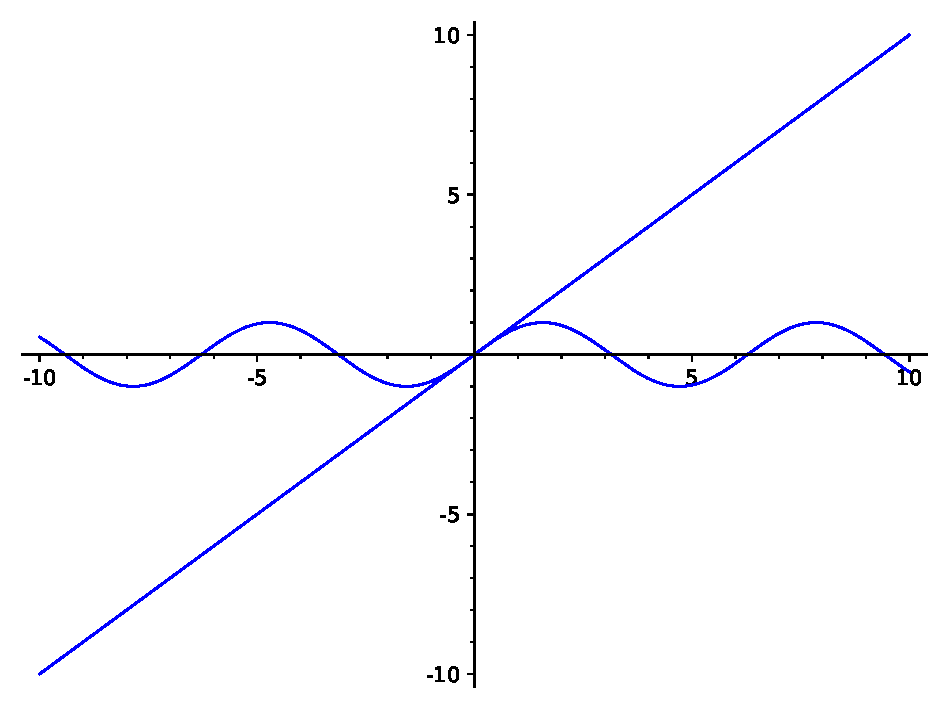
\includegraphics{cviceni_8/fig/taylor_sin_1.pdf}
				\caption{$\sin(x)$ vs $T(x) = x$}
				\label{fig:taylor_1_sin}
			\end{figure}
			\begin{figure}[H]
				\centering
				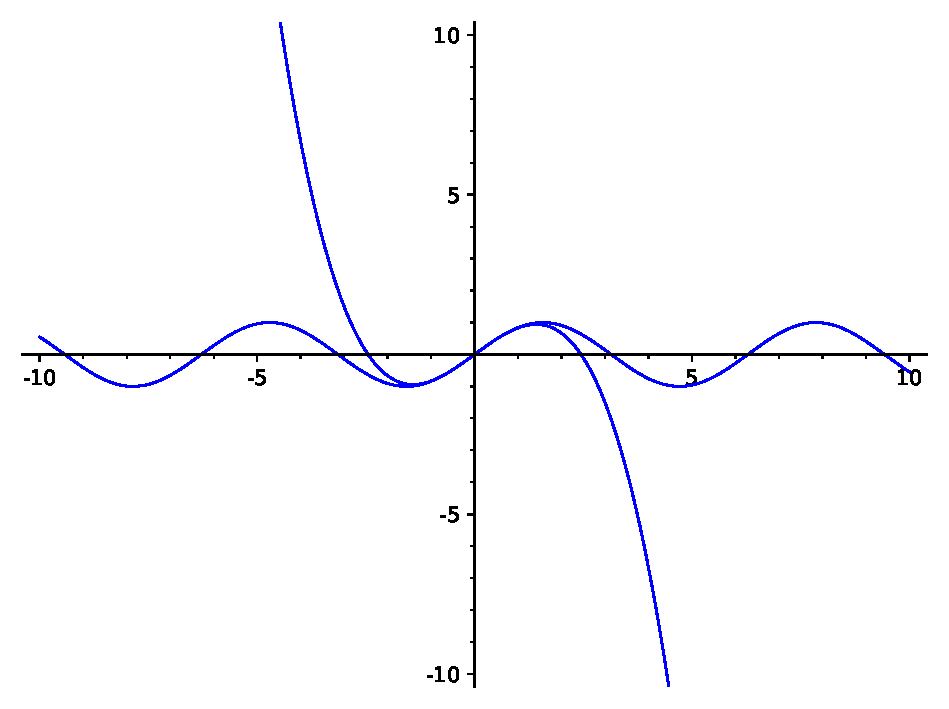
\includegraphics{cviceni_8/fig/taylor_sin_3.pdf}
				\caption{$\sin(x)$ vs $T(x) = x - \frac{x^3}{3!}$}
				\label{fig:taylor_3_sin}
			\end{figure}
			\begin{figure}[H]
				\centering
				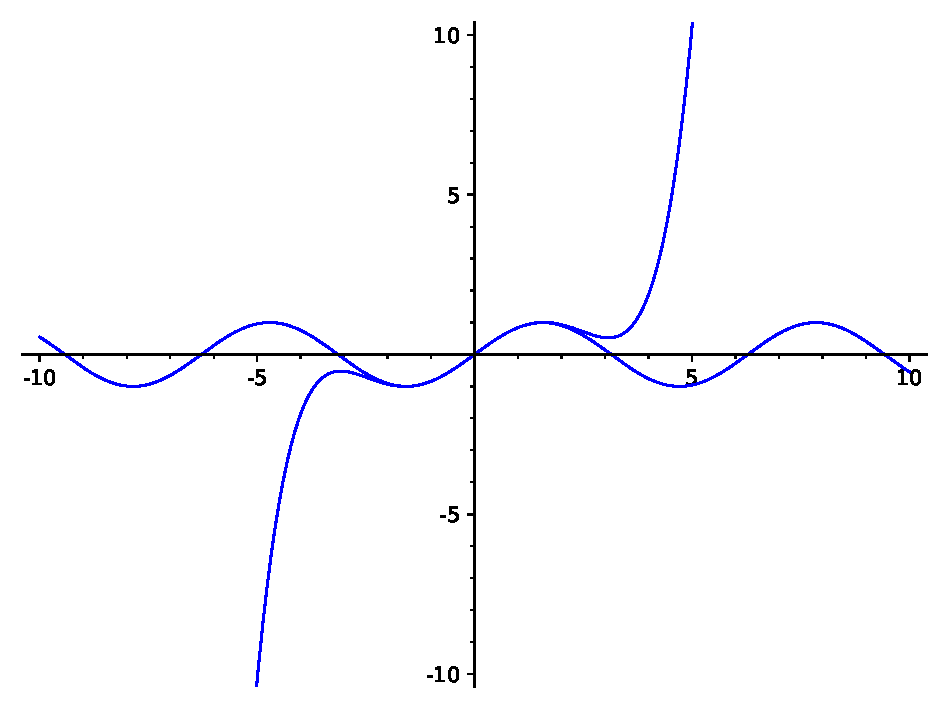
\includegraphics{cviceni_8/fig/taylor_sin_5.pdf}
				\caption{$\sin(x)$ vs $T(x) = x - \frac{x^3}{3!} + \frac{x^5}{5!}$}
				\label{fig:taylor_5_sin}
			\end{figure}
			\begin{figure}[H]
				\centering
				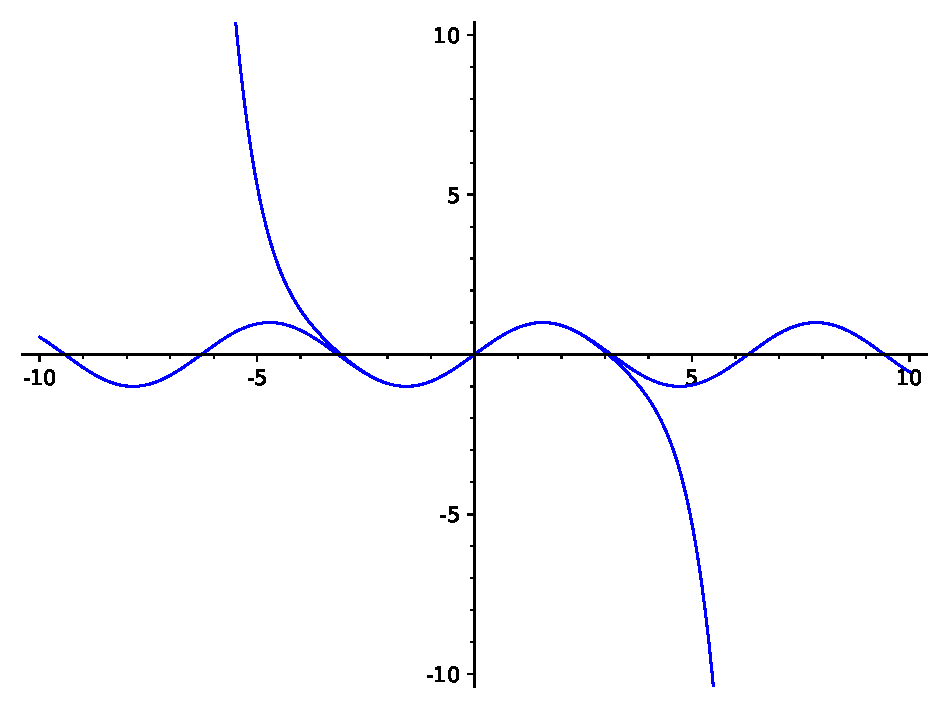
\includegraphics{cviceni_8/fig/taylor_sin_7.pdf}
				\caption{$\sin(x)$ vs $T(x) = x - \frac{x^3}{3!} + \frac{x^5}{5!} - \frac{x^7}{7!}$}
				\label{fig:taylor_7_sin}
			\end{figure}
			\begin{figure}[H]
				\centering
				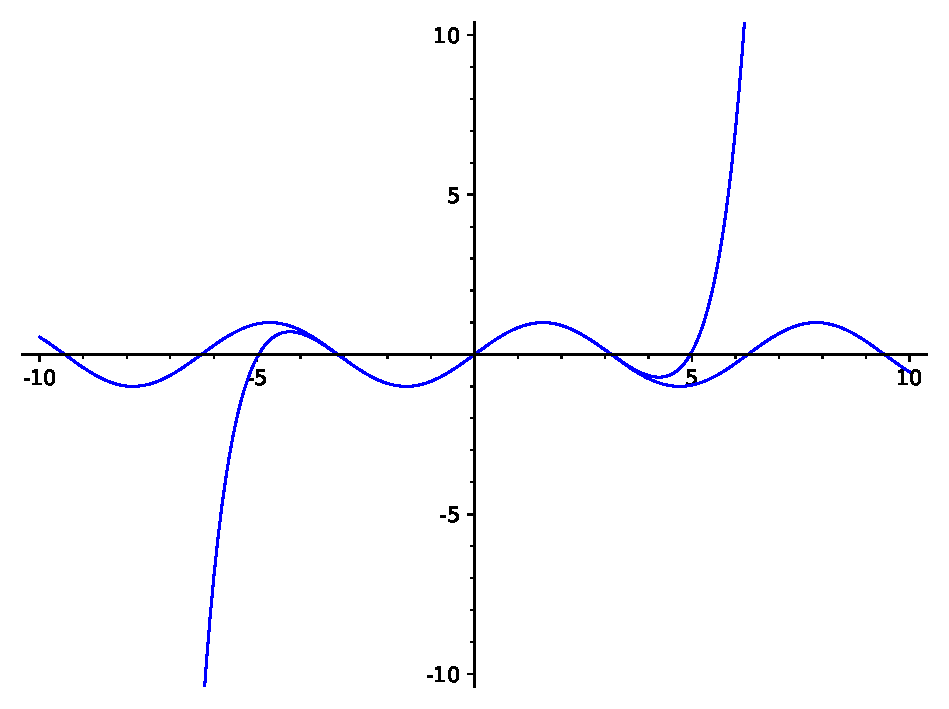
\includegraphics{cviceni_8/fig/taylor_sin_9.pdf}
				\caption{$\sin(x)$ vs $T(x) = x - \frac{x^3}{3!} + \frac{x^5}{5!} - \frac{x^7}{7!} + \frac{x^9}{9!}$}
				\label{fig:taylor_9_sin}
			\end{figure}
			\begin{figure}[H]
				\centering
				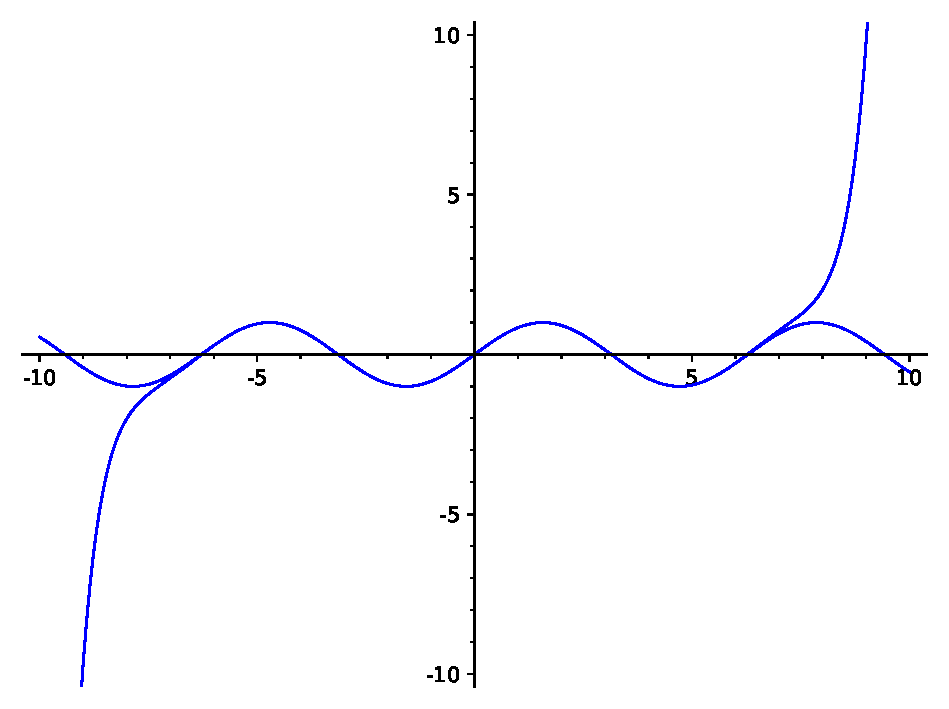
\includegraphics{cviceni_8/fig/taylor_sin_17.pdf}
				\caption{$\sin(x)$ vs $T(x) = x - \frac{x^3}{3!} + \frac{x^5}{5!} - \frac{x^7}{7!} + \frac{x^9}{9!} - \frac{x^{11}}{11!} + \frac{x^{13}}{13!} - \frac{x^{15}}{15!} + \frac{x^{17}}{17!}$}
				\label{fig:taylor_17_sin}
			\end{figure}
		}

\end{enumerate}

